%!TEX root=../../root.tex

\section{Lezione 4}
\subsection{Algoritmi di problemi di riduzione}
\subparagraph{Algoritmo per linguaggio vuoto in DFA}
\begin{description}
	\item \emph{Input:} $A = (Q, \Sigma, \delta, q_0, F) \in DFA$
	\item \emph{Output:} s\`i se $L(A)=\emptyset$, no altrimenti
	\item \emph{Algoritmo:}\newline
		\begin{enumerate}
			\item Costruisci il grafo diretto $G=(V,E)$ cos\`i definito:
			\[
				V = Q \cup \{t | t \notin Q \}
			\]
			\[
				E = \{(p,q) | p, q \in Q \land \exists a \in \Sigma \land \delta(p, a) = q \} \cup \{(p,t) | p \in F\}			
			\]
			\item Verificare se c'\`e un cammino da $q_0$ a $t$; se s\`i rispondi no ($L(A)$ non vuoto), altrimenti rispondi s\`i
		\end{enumerate}
	\item \emph{Complessit\`a:} $\Theta (|Q|+|Q|\times|\Sigma|)$.
\end{description}
\subparagraph{Algoritmo per linguaggio finito in DFA}
\begin{description}
	\item \emph{Input:} $A = (Q, \Sigma, \delta, q_0, F) \in DFA$
	\item \emph{Output:} s\`i se $L(A)$ \`e finito, no altrimenti
	\item \emph{Algoritmo:}
		\begin{enumerate}
			\item Costruisci il grafo $G=(V,E)$ cos\`i definito:
			\[
				V = Q			
			\] 
			\[
				E = \{(p,q) | p, q \in Q \land \exists a \in \Sigma \delta(p,a) = q\}
			\]
			\item Elimina i nodi non raggiungibili da $q_0$ o dai quali non si raggiunge un nodo corrispondente ad uno stato finale.
			\item Verifica se G \`e aciclico; se s\`i rispondi s\`i ($L(A)$ \`e finito), altrimenti rispondi no.
	\item \emph{Complessit\`a:} $\Theta (|Q|+|Q|\times|\Sigma|)$.
		\end{enumerate}
\end{description}
\subsection{Definizione formale di NFA }
Possiamo definire un automa non deterministico esattamente come abbiamo fatto per gli automi deterministici, quello che cambia \`e la definizione della funzione $\delta$. Quindi un NFA \`e una quintupla $(Q, \Sigma, \delta, q_0, F)$ tale che: 
\[
	\delta : Q \times \Sigma \to {\cal P} (Q)
\]
Ossia $\delta (q,a) ={\cal P} (Q)$, quindi preso uno stato di partenza in $Q$ e un carattere $a \in \Sigma$ la funzione stabilisce in quale insieme di stati pu\`o transitare l'automa dopo la lettura di $a$. \newline
Notare che i $DFA$ sono casi particolari di $NFA$, ossia $NFA$ con stati singoletto.
\subsection{Da NFA a DFA}
Dopo aver capito l'utilit\`a di costruire automi non deterministici ci chiediamo se esiste un modo formale per costruire un automa deterministico partendo da un automa non deterministico.
\subparagraph{Teorema}
$	\forall A = (Q, \Sigma, \delta, q_0, F) \in NFA$ $\exists A'= (Q', \Sigma, \delta', q'_0, F') \in DFA$ tale che:
\begin{description}
	\item $Q' =  {\cal P}(Q)$
	\item $\forall X \in {\cal P}(Q)$ $\delta'(X,a) = \bigcup_{p \in X} \delta(p, a)$
	\item $q_0 = \{q_0\}$
	\item $F' = \{ X | X \in {\cal P}(Q) \land X \cap F \neq 0\}$
\end{description}
Notare che $|Q'| = 2^{|Q|}-1$.
\subparagraph{Algoritmo}
\begin{description}
	\item \emph{Input:} $A = (Q, \Sigma, \delta, q_0, F) \in NFA$
	\item \emph{Output:} $A' = (Q', \Sigma, \delta', q'_0, F') \in DFA$
	\item \emph{Algoritmo:}
		\begin{enumerate}[label*=\arabic*.]
			\item Poni $Q' = \{\{q_0\}\}$
			\item Ripeti finch\`e in $Q'$ ci sono stati non marcati
				\begin{enumerate}[label*=\arabic*.]
					\item Prendi un elemento non marcato $X \in Q'$
					\item Marca X
					\item $\forall a \in \Sigma$
						\begin{enumerate}[label*=\arabic*.]
							\item $Y_a = \bigcup_{p \in X} \delta(p,a)$
							\item $\delta'(X,a) = Y_a$
							\item $Y_a \notin Q' \Rightarrow$ aggiungi $Y_a$, non marcato, in $Q'$  						
						\end{enumerate}
					\item $\delta'(X,a)=Y$
					\item $Y \notin Q' \Rightarrow$ aggiungi $Y$, non marcato, a $Q'$
		
				\end{enumerate}
			\item $\forall X \in {\cal P}(Q) - Q'$ $\delta'(X, a) = \emptyset$ $ \forall a \in \Sigma$. Questo serve per rendere $\delta$ completo.
			\item Poni $q_0 = \{ q_0\}$ e $F' = \{X \in {\cal P}(Q) | X \cap F \neq \emptyset\}$
		\end{enumerate}
\end{description}

\subparagraph{Esempio}
Automa $A$ tale che $L(A) = \{x1ab | x 	\in \Sigma^{\star}\land a, b \in \Sigma \}$.
\begin{description}
	\item \emph{$NFA$:}
		\begin{figure}[H]
			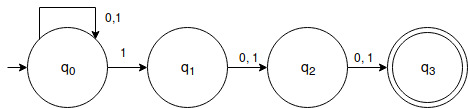
\includegraphics[scale=0.6]{nfadfa}
		\end{figure}
	\item \emph{$DFA$:}
		\begin{figure}[H]
			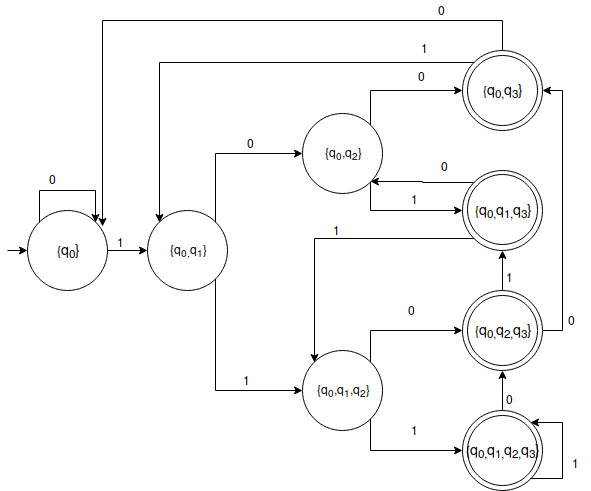
\includegraphics[scale=0.6]{nfadfa2}
		\end{figure}
\end{description}
\subsection{NFA con $\varepsilon$ mosse}
Vorremmo essere in grado di poter rappresentare dei cambi di stato non determinati da alcun input. Per far ci\`o usiamo la parola vuota. Pi\`u formalmente: 
\[
	A = (Q, \Sigma_{\varepsilon}, \delta, q_0, F)
\]
Dove:
\[
	\Sigma_{\varepsilon} = \Sigma \cup \{\varepsilon\}
\]
\[
	\delta : Q \times \Sigma_{\varepsilon} \to {\cal P}(Q)
\]
\begin{description}
	\item \emph{Esempio 1:} Ricerca stringhe nel testo. Sia $\Sigma = \{$ alfabeto inglese $\}$ vogliamo definire un $NFA$ $A$ tale che $L(A) = \{$ color, colour, web $\}$.
	\begin{figure}[H]
		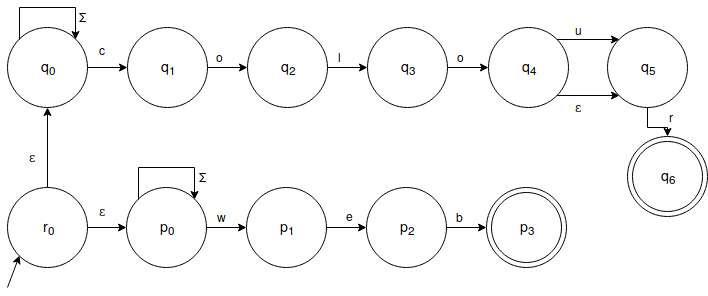
\includegraphics[scale=0.6]{nfa2}
	\end{figure}
	\item \emph{Esercizio 1:} Automa che riconosce i numeri reali.
\end{description}

